\chapter*{Part A:\@ Classification}

\section*{Introduction}

The Landsat satellites are part of a continuous effort between NASA and
the US Geological Survey to acquire land remote sensing data. The
Multispectral Scanner (MSS) sensor aboard the satellites acquires imagery
of the earth in four different spectral bands --- two of these are in the
visible region (corresponding approximately to green and red regions of
the visible spectrum) and two are in the (near) infra-red.

The database consists of the multi-spectral values of pixels in 3\(\times \)3
neighbourhoods in a satellite image, and the classification associated with
the central pixel in each neighbourhood. The aim is to predict this
classification, given the multi-spectral values. 

The whole data set contains 6435 lines. In each line, the multi-spectral
values of a neighborhood are specified: the four values for the top-left
pixel are given first, followed by the top-middle pixel and then the
top-right pixel, and so on with the pixels read out in sequence
left-to-right and top-to-bottom. These multi-spectral values are
integer-coded from 0 (black) to 255 (white). The class value of the centre
pixel is coded as another integer:

\begin{center}
\begin{tabular}{cc}
    Integer & Class \\
    \midrule
    1 & red soil \\ 
    2 & cotton crop \\
    3 & grey soil \\
    4 & damp grey soil \\
    5 & soil with vegetation stubble \\
    6 & mixture class (all types present) \\
    7 & very damp grey soil \\
\end{tabular}
\end{center}

No line of class 6 is present in the data set. The training set contains
4435 lines, while the testing set contains 2000 lines.

Multilayer feed-forward neural networks are suitable to solve classification
problems like this, because it can approximate an arbitrary nonlinear
function to a high degree of accuracy, given enough training data.

\section*{Experiments}

We implemented the neural network as a function \texttt{train\_test\,()}
taking three optional parameters: 
\texttt{batch\_size}, \texttt{hl\_neuron} (the hidden layer neuron count) and
\texttt{decay}. Each experiment is performed by utilizing the search function
\texttt{search\,()}, which takes two additional inputs, the search parameter
(either \texttt{batch\_size}, \texttt{hl\_neuron} or \texttt{decay}) and the
search space associated with it. The function would loop through the possible
values of the parameter, and train and test the neural network accordingly;
graphs are stored and displayed after each experiment.

\subsection*{Experiment 1: Determining the optimal batch size (Question 2)}

The parameter \texttt{batch\_size} is varied in the search space
\([4,8,16,32,64]\).
Plotting the training errors against the number of epochs for different
batch sizes:

\begin{center}
    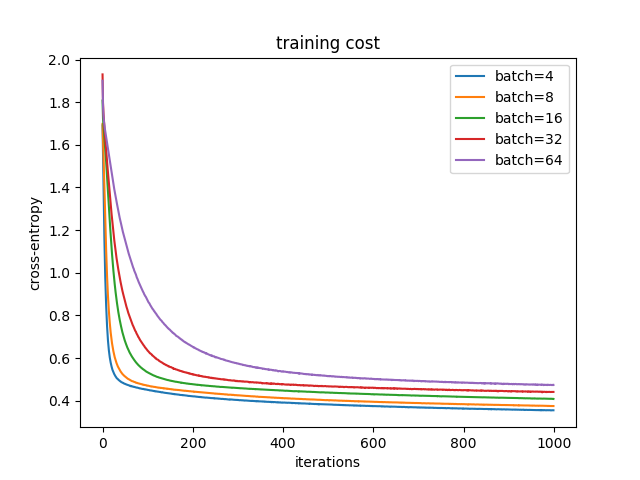
\includegraphics[width=\imgw]{images/p1a2_batch_cost.png}   
\end{center}

Plotting the test accuracy against the number of epochs for different
batch sizes:

\begin{center}
    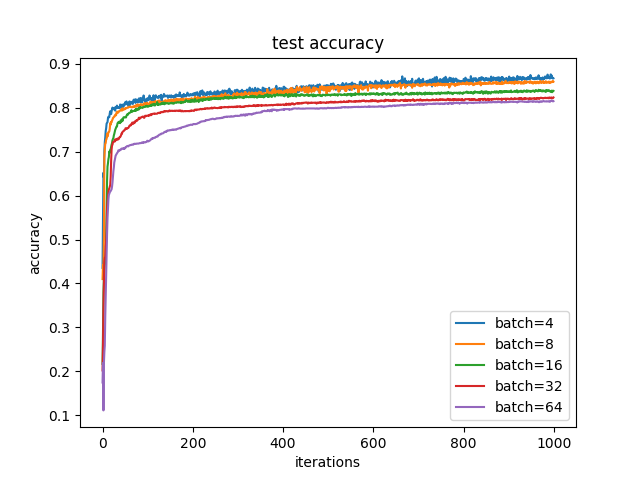
\includegraphics[width=\imgw]{images/p1a2_batch_accuracy.png}   
\end{center}

Plotting the time taken to update parameters for different batch sizes:

\begin{center}
    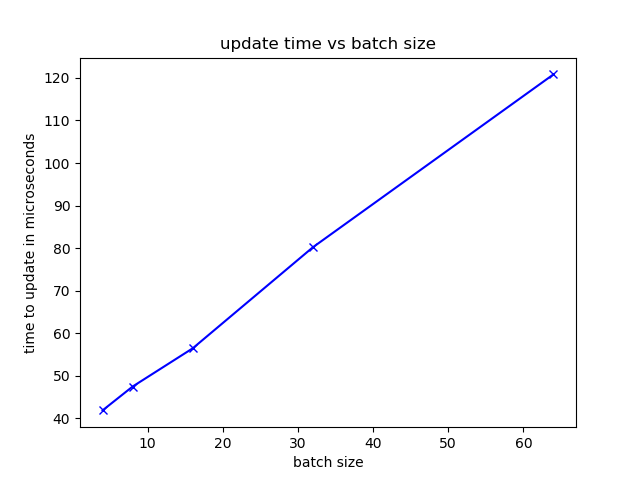
\includegraphics[width=\imgw]{images/p1a2_batch_times.png}   
\end{center}

We decided to choose batch size of 4, for the highest test accuracy. 

\subsection*{Experiment 2: Determining the optimal number of hidden neurons
(Question 3)}

The parameter \texttt{hl\_neuron} is varied in the search space
\([5,10,15,20,25]\).
Plotting the training errors against the number of epochs for different hidden
neuron counts:

\begin{center}
    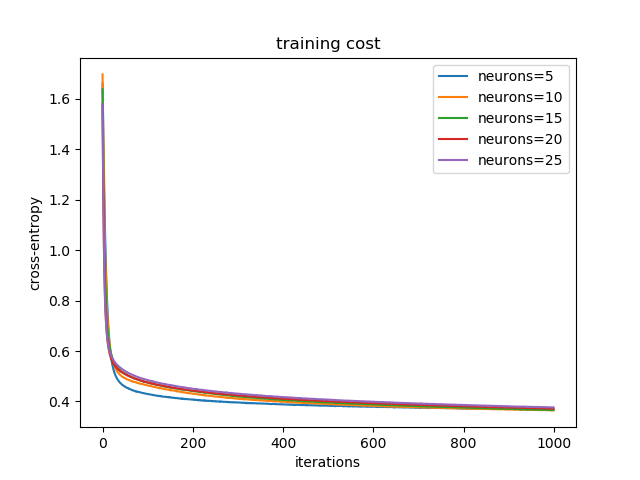
\includegraphics[width=\imgw]{images/p1a3_neuron_cost.png}   
\end{center}

Plotting the test accuracy against the number of epochs for different hidden
neuron counts:

\begin{center}
    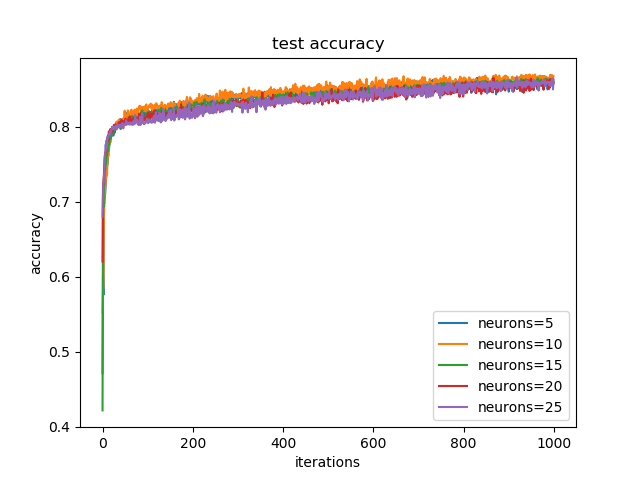
\includegraphics[width=\imgw]{images/p1a3_neuron_accuracy.png}   
\end{center}

Plotting the time taken to update parameters for different hidden neuron counts:

\begin{center}
    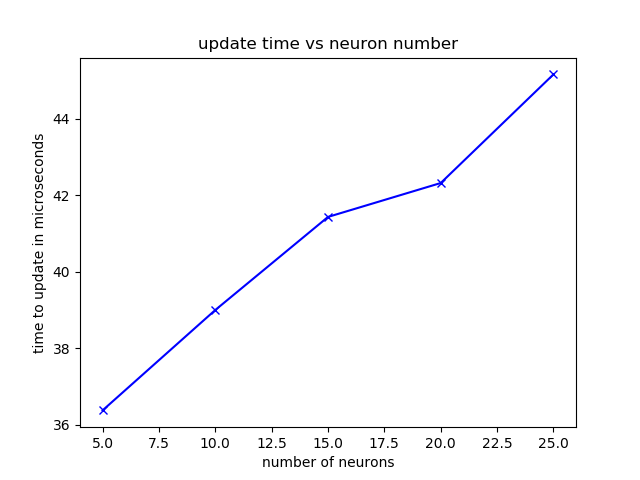
\includegraphics[width=\imgw]{images/p1a3_neuron_times.png}   
\end{center}

We decided to choose 10 hidden neurons, for the highest test accuracy.

\subsection*{Experiment 3: Determining the optimal decay parameter (Question 4)}

The parameter \texttt{decay} is varied in the search space
\([0, 10^{-12}, 10^{-9}, 10^{-6}, 10^{-3}]\).
Plotting the training errors against the number of epochs for different decay
parameters:

\begin{center}
    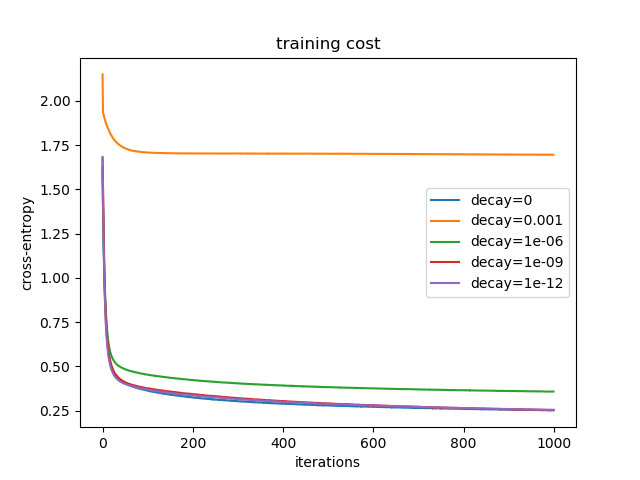
\includegraphics[width=\imgw]{images/p1a4_decay_cost.png}   
\end{center}

Plotting the test accuracy against the decay parameters:

\begin{center}
    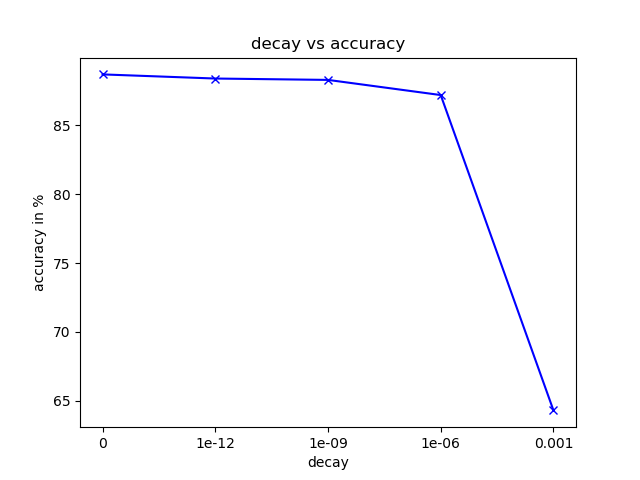
\includegraphics[width=\imgw]{images/p1a4_decay_accuracy.png}   
\end{center}

We decided to choose decay parameter \(10^{-9}\), for the highest accuracy.

\subsection*{Experiment 4: The 4-layer neural network (Question 4)}

Plotting the training errors against the number of epochs for the 4-layer
network:

\begin{center}
    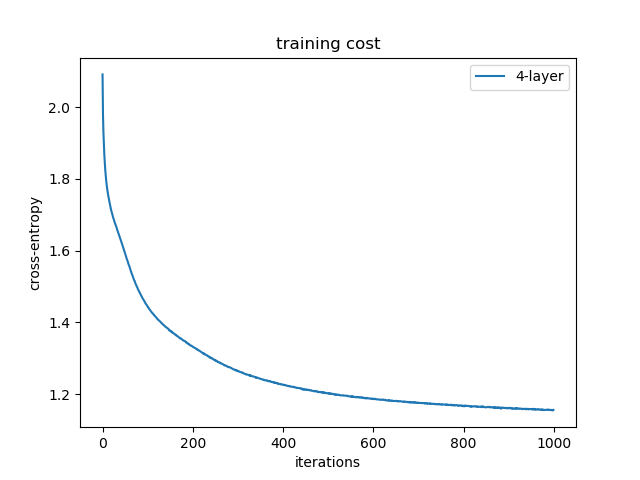
\includegraphics[width=\imgw]{images/p1a5_4-layer_cost.png}   
\end{center}

Plotting the test accuracy against the number of epochs for the 4-layer
network:

\begin{center}
    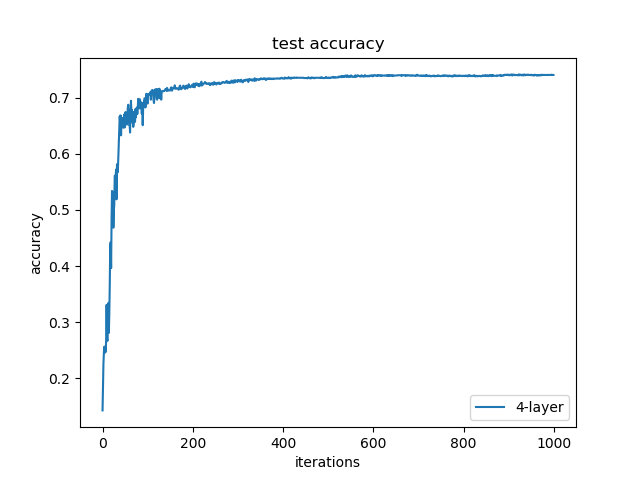
\includegraphics[width=\imgw]{images/p1a5_4-layer_accuracy.png}   
\end{center}

The 3-layer network achieves a higher accuracy compared to the 4-layer
network. This shows that more layers do not neccesarily lead to higher
performance in a feedforward neural network.
